\documentclass[a4paper]{article}
\usepackage{amsfonts}
\usepackage{amsmath}
\usepackage{amssymb}
\usepackage{graphicx}     
\newcommand{\ddx}{\dfrac{d}{dx}}
\newcommand{\ddg}{\dfrac{d}{dg}}
\begin{document}
  
\noindent \large Auteur: Luca Letroye \\
\noindent \large Studierichting: Informatica\\
\noindent \large Oefeningenreeks 3G nr. 2\\

\medskip


\normalsize

$ f(x) = (x-2)^3 +1 $ \\

$f(x) = x^3-6x^2+12x-7$\\

\begin{tabular}{c|ccc||c} 
    & $1$ & $-6$ & $12$ & $-7$ \\ 
    $1$ & $\downarrow$ & $1$ & $-5$ & $7$ \\ \hline
    $$ & 1 & -5 & 7 & 0  \\
\end{tabular}\\

$f(x) = (x-1)(x^2-5x +7)$\\

$D = (-5)^2-4\cdot 1\cdot 7 = -3 \Rightarrow \text{geen nulpunten}$\\

$f'(x) = 3x^2-12x+12$\\

$D = (-12)^2-4\cdot 3\cdot 12 = 0$\\

$x = \dfrac{-b}{2a} = \dfrac{12}{6} = 2$\\

$f'(1) = 3 \Rightarrow y-0 = 3(x-1)$\\

$y = 3x-3$\\

$f''(x) = 6x - 12 \Rightarrow 6x - 12 = 0$\\

$x = 2$\\

$\operatorname{dom}f = \mathbb{R} $\\

asymptoten: geen\\

\begin{tabular}{c|ccccc} 
    & $$ & $1$ & $$ & $2$ & $$ \\ \hline
    $f(x)$ & $-$ &  $0$ & $+$ & $+$ & $+$\\
    $f'(x)$ & $+$ &  $+$ & $+$ & $0^{(2)}$ & $+$\\
    $f(x)$ & $\nearrow$ &  $\nearrow$ & $\nearrow$ & $1$ & $\nearrow$\\
    $f''(x)$ & $-$ &  $-$ & $-$ & $0$ & $+$\\
    $f(x)$ & $\frown$ &  $\frown$ & $\frown$ & $B$ & $\smile$\\
\end{tabular}\\

\begin{figure}[h]
\centering
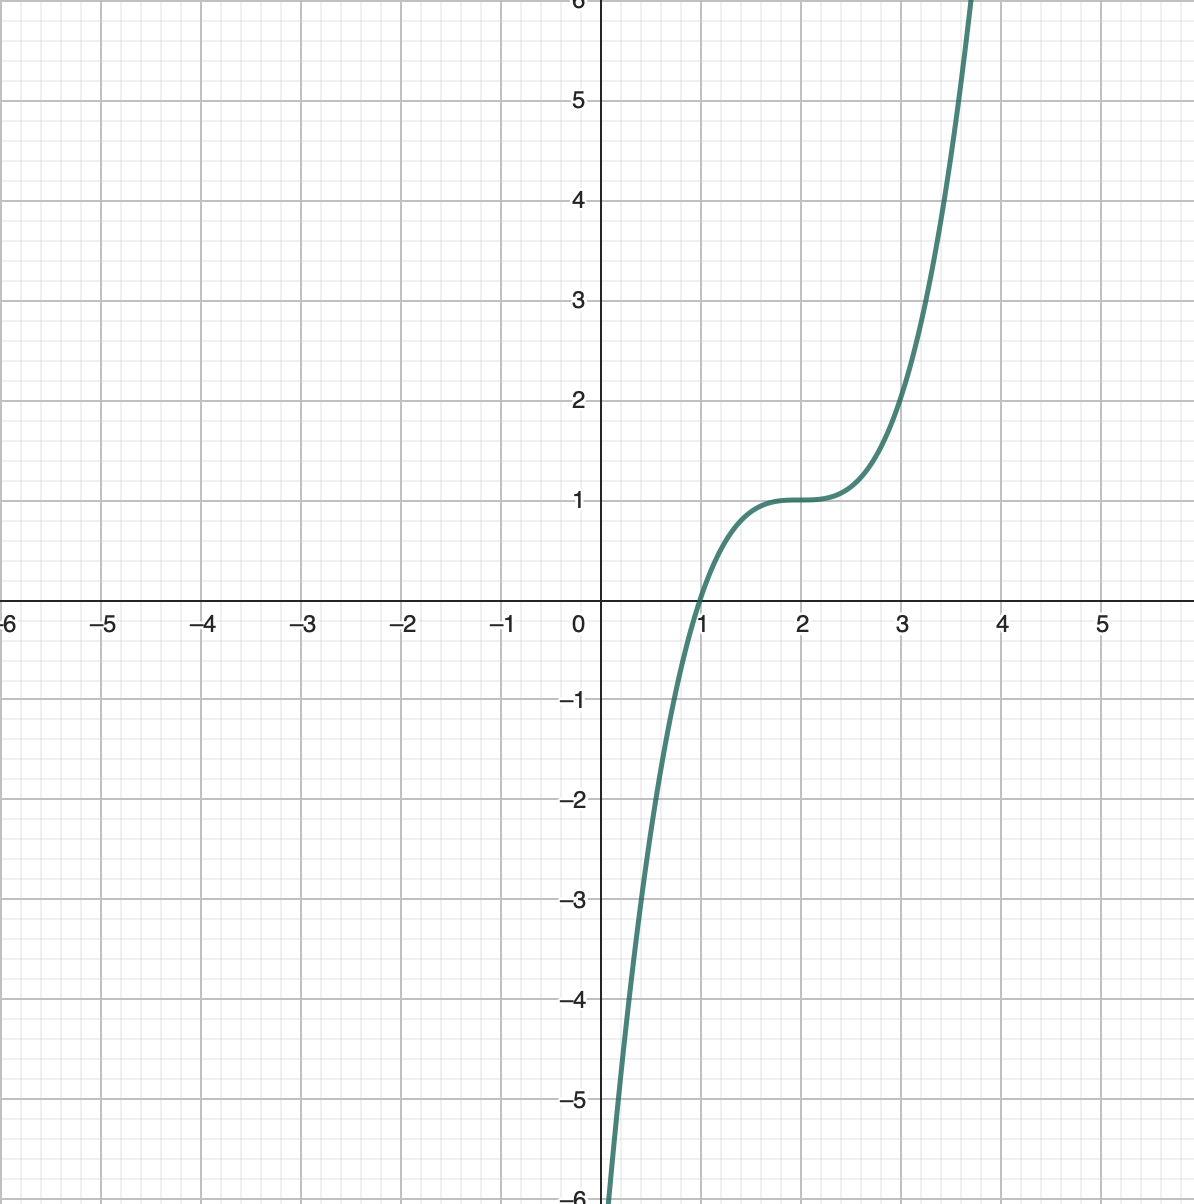
\includegraphics[width=10cm]{3G-2-luca.letroye.INF.png}
\end{figure}







\begin{thebibliography}{999}
%\bibitem{a} Referentie
\end{thebibliography}
\end{document} 
